%% Template for a preprint Letter or Article for submission
%% to the journal Nature.
%% 
%%

\documentclass[11pt]{article}
\usepackage[margin=1in]{geometry}
\usepackage{graphicx}
\usepackage{amsfonts}
\usepackage{etoolbox}
\usepackage{adjustbox}
\usepackage{amsmath}
\usepackage{setspace}
\usepackage{textcomp}
\usepackage{geometry}
\usepackage{amssymb}
\usepackage{wrapfig}
\usepackage{rotating}
\usepackage{changepage}
\usepackage{longtable}
\usepackage[document]{ragged2e}
\usepackage{lscape}
\usepackage{lineno}
\linenumbers
\usepackage{float}
\floatplacement{figure}{H}



%% make sure you have the nature.cls and naturemag.bst files where
%% LaTeX can find them

\bibliographystyle{naturemag}

\title{ENSO increases foreign fishing\footnote{Work in progress; do not circulate.}}

%% Notice placement of commas and superscripts and use of &
%% in the author list

\author{ Kimberly L. Oremus$^{1}$*, Juan Carlos Villase\~{n}or-Derbez$^{1}$*}


\begin{document}
\doublespacing
\maketitle

\begin{enumerate}
 \item Bren School of Environmental Science and Management, University of California, Santa Barbara.
\end{enumerate}
* In alphabetical order for now, but we should chat about authorship.

\begin{abstract}
Illegal, unreported and unregulated (IUU) fishing contributes to x\% of the global fishing ecconomy \cite{Agnew:2009}. Foreign fishing in a nation's Exclusive Economic Zone (EEZ) contributes to a y\% of IUU fishing \cite{Cabral:2018}. Drivers of foreign fishing include a, b and c, but it is unclear how this may change under climate change. We show ENSO events increase foreign fishing by z\%. We also find the effect is lower for more adaptive gears such as longliners. This quantitative evidence linking climate and fishing behavior have important implications for climate projections and adaptation of this sector.
%This effect is larger for vessels with less fishing experience and lower for vessels with higher fishing experience.
\end{abstract}

\newpage

\section{Introduction}

Fisheries are an important souce of food, livelihoods, local and national economies \cite{SOFIA:2018}. A growing body of literature highlights how climate impacts could reduce catch \cite{Sumaila:2011, Lam:2016} and theoretically incentize overfishing or illegal fishing as stocks shift their distributions \cite{Pinsky:2018}. Empirical evidence has been limited to case studies (CITE). However, advances in technology allow us to understand fishing behavior \cite{Kroodsma:2018, Cabral:2018, McDermott:2018}. 

Satellite data using an automatic identification system (AIS) allows us to see where individual boats go, and infer when fishing events occur \cite{ Kroodsma:2018}. Recent studies have captured how policies, such as banning foreign fishing \cite{Cabral:2018} and the creation of Marine Protected Areas have impacted illegal, unreported and unregulated fishing (IUU) \cite{McDermott:2018}. The high-resolution data also lends itelf well to exploring how the physical environment impacts fishing behavior.

There is a large literature on how highly migratory stocks such as tuna move with sea-surface temperatures \cite{aqorau:2018} and has been empirically shown to move during El Ni\~{n}o and La Ni\~{n}a events \cite{lehodey:1997}. Theoretically fishing fleets could follow the stocks. However, limitations in fishing jurisidictions such as Exlusive Economic Zones (EEZ) and Marine Protected Areas (MPAs-SHOULD WE EXPAND THE ANALYSIS TO MPAs) may impact their decisions on where to fish. We do not know if fishing fleets tend to reduce fishing during El Ni\~{n}o/La Ni\~{n}a, or make the costly decision to increase fishing in foreign waters (and protected areas). 

Using publically available data through the Global Fishing Watch (GFW) initiative,we document how purse seine and longline fleets respond to El Ni\~{n}o and La Ni\~{n}a years, where local environmental conditions are more extreme. We do this by segmenting the ocean into treatment and control regions, where treatment regions are regions whose local environmental variables are correlated to ENSO and control regions have no correlation between the local environment and ENSO (See Methods~\ref{Treatment}). We then compare the number of hours vessels fish in foreign waters during neutral ENSO months to El Nino and La Nina months in treatment regions and control regions (See Methods~\ref{ENSO_FF}).  

\clearpage

\section{Results}
Let's go through the results

\begin{figure}
\centering
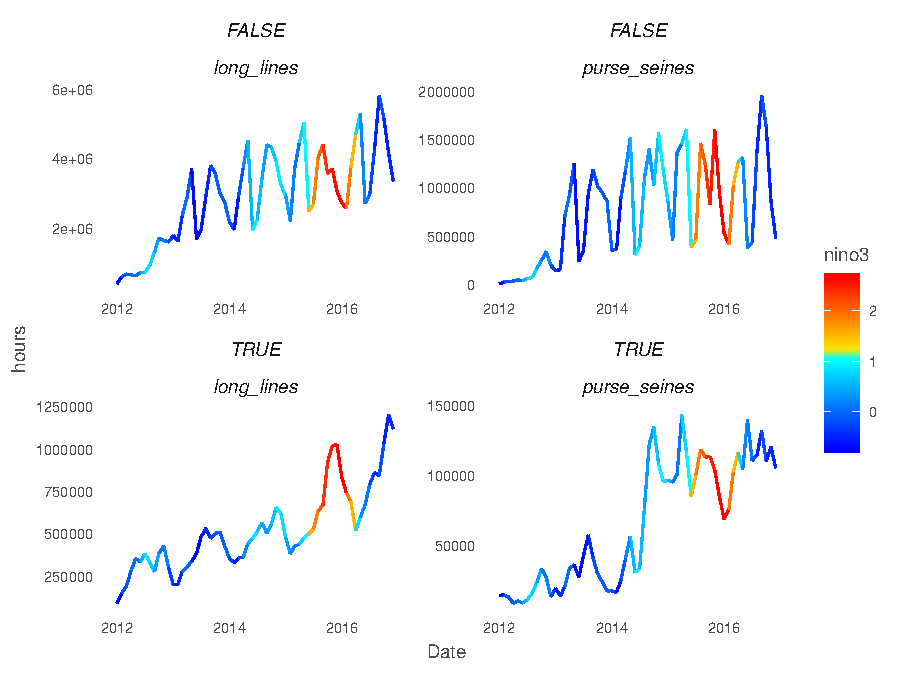
\includegraphics{img/trends_by_gear.pdf}
\caption{Trends in fishing hours by gear and foreign}
\end{figure}

\begin{figure}
\centering
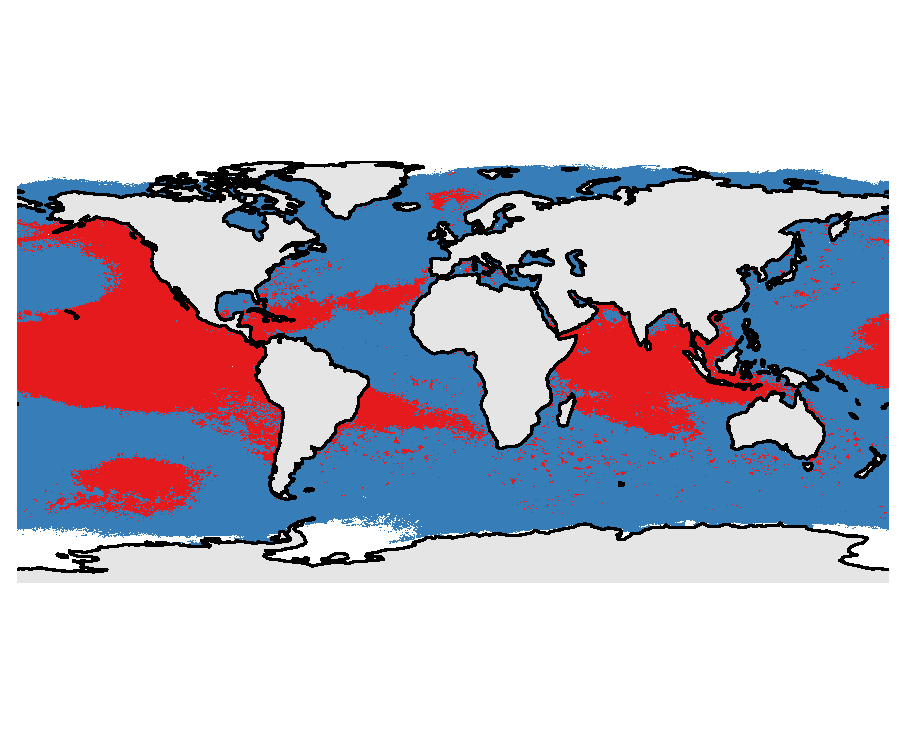
\includegraphics{img/teleconnected_3months.pdf}
\caption{ENSO-teleconnected Ocean Regions}
\end{figure}

\clearpage

\begin{table}[!htbp] \centering 
  \caption{\label{tab:ff_reg}Effect of NINO3.4 anomally index on foreign fishing for purse seiners (1-3) and longliners(4-6).} 
  \label{} 
\begin{tabular}{@{\extracolsep{5pt}}lcccccc} 
\\[-1.8ex]\hline 
\hline \\[-1.8ex] 
 & \multicolumn{6}{c}{\textit{Dependent variable:}} \\ 
\cline{2-7} 
\\[-1.8ex] & \multicolumn{6}{c}{Monthly foreign fishing hours} \\ 
\\[-1.8ex] & (1) & (2) & (3) & (4) & (5) & (6)\\ 
\hline \\[-1.8ex] 
 nino34anom & $-$0.010$^{***}$ & $-$0.011$^{***}$ & $-$0.014$^{***}$ & 0.013$^{***}$ & 0.015$^{***}$ & 0.015$^{***}$ \\ 
  & (0.001) & (0.001) & (0.001) & (0.001) & (0.001) & (0.001) \\ 
  & & & & & & \\ 
 treated & $-$0.176$^{***}$ & $-$0.170$^{***}$ & 0.031$^{***}$ & $-$0.021$^{***}$ & $-$0.016$^{***}$ & $-$0.086$^{***}$ \\ 
  & (0.001) & (0.001) & (0.003) & (0.001) & (0.001) & (0.002) \\ 
  & & & & & & \\ 
 nino34anom:treated & 0.069$^{***}$ & 0.070$^{***}$ & 0.077$^{***}$ & 0.031$^{***}$ & 0.027$^{***}$ & 0.031$^{***}$ \\ 
  & (0.001) & (0.001) & (0.001) & (0.002) & (0.002) & (0.002) \\ 
  & & & & & & \\ 
 Constant & 1.177$^{***}$ & 1.120$^{***}$ & 2.132$^{***}$ & 1.318$^{***}$ & 1.297$^{***}$ & 2.303$^{***}$ \\ 
  & (0.001) & (0.002) & (0.042) & (0.001) & (0.002) & (0.113) \\ 
  & & & & & & \\ 
\hline \\[-1.8ex] 
Month FE & No & Yes & Yes & No & Yes & Yes \\ 
Country FE & No & No & Yes & No & No & Yes \\ 
Observations & 3,819,575 & 3,819,575 & 3,819,575 & 5,086,606 & 5,086,606 & 5,086,606 \\ 
R$^{2}$ & 0.005 & 0.006 & 0.023 & 0.0003 & 0.002 & 0.026 \\ 
\hline 
\hline \\[-1.8ex] 
\textit{Note:}  & \multicolumn{6}{r}{$^{*}$p$<$0.1; $^{**}$p$<$0.05; $^{***}$p$<$0.01} \\ 
\end{tabular} 
\end{table} 

\begin{table}[!htbp] \centering 
  \caption{\label{tab:ff_reg}Effect of NINO3.4 anomally index on foreign fishing for purse seiners (1-3) and longliners(4-6).} 
  \label{} 
\begin{tabular}{@{\extracolsep{5pt}} c} 
\\[-1.8ex]\hline 
\hline \\[-1.8ex] 
TRUE \\ 
\hline \\[-1.8ex] 
\end{tabular} 
\end{table} 

\clearpage

\begin{figure}
\centering
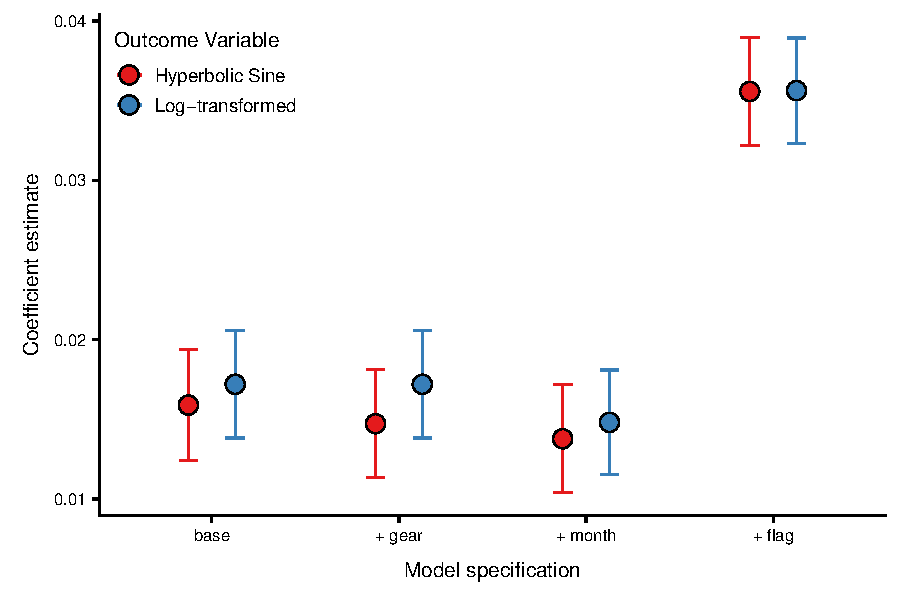
\includegraphics{img/coef_estimates.pdf}
\caption{Coefficient estimates for the models ran above. Graphs on the left show estimates after the hyperbolic sine transformation of hours. Right side show no transformation of hours.
 Model numbers (x - axis) correspond to the columns in table 1 (1 - 4) and table 2 (5 - 8).}
\end{figure}

\section{Discussion}

Purse seiners: More regulation, gear can't go as deep
Long-liners: Less regulated, but gear can go deeper 
Trawlers: Are species as impacted by ENSO events?


\subsection{Methods}

\subsubsection{Global Fishing Watch data}

\begin{figure}
\centering
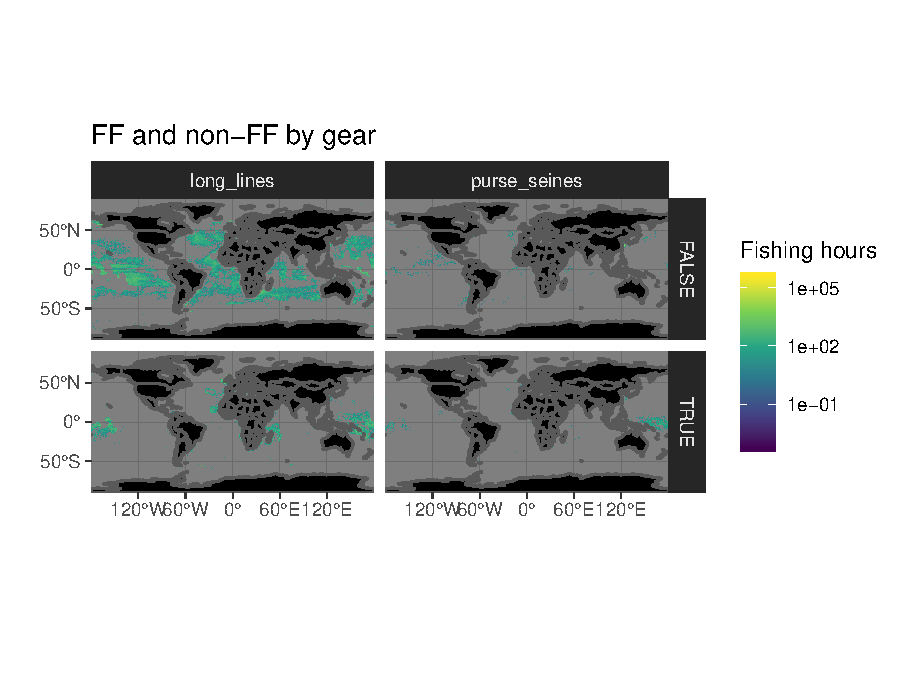
\includegraphics{img/fishing_raster.pdf}
\caption{Fishing effort (hours) by gear and foreign fishing}
\end{figure}


\subsubsection{El Ni\~{n}o-Southern Oscillation}

\begin{figure}
\centering
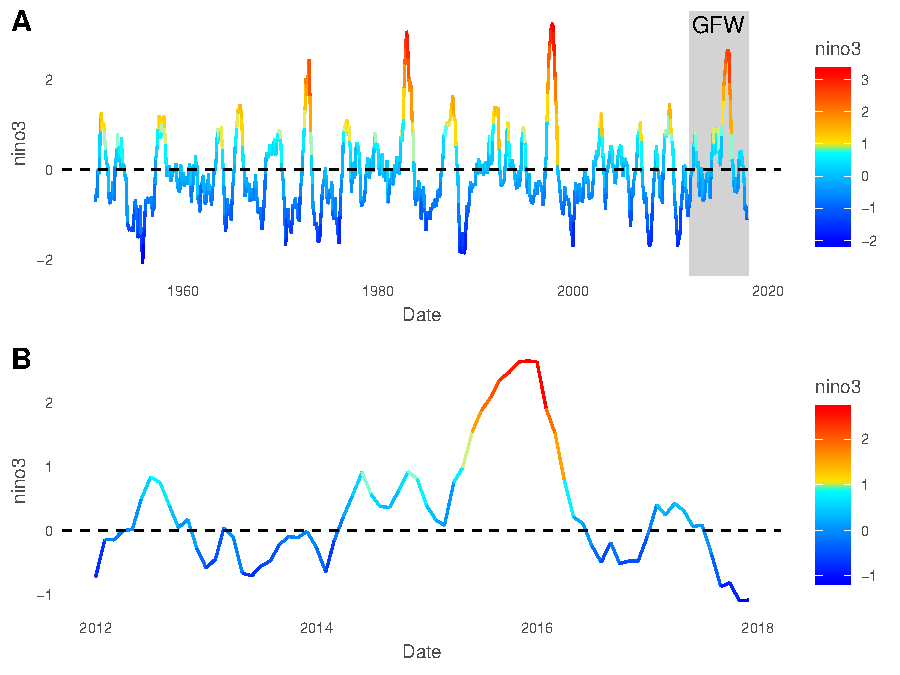
\includegraphics{img/nino_gfw.pdf}
\caption{Timeseries of nino3 index (detrended) for A) The entire length
and B) timespan matching GFW data}
\end{figure}

\subsubsection{Empirical specifications: ENSO and Foreign Fishing}
\label{ENSO_FF}

\begin{figure}
\centering
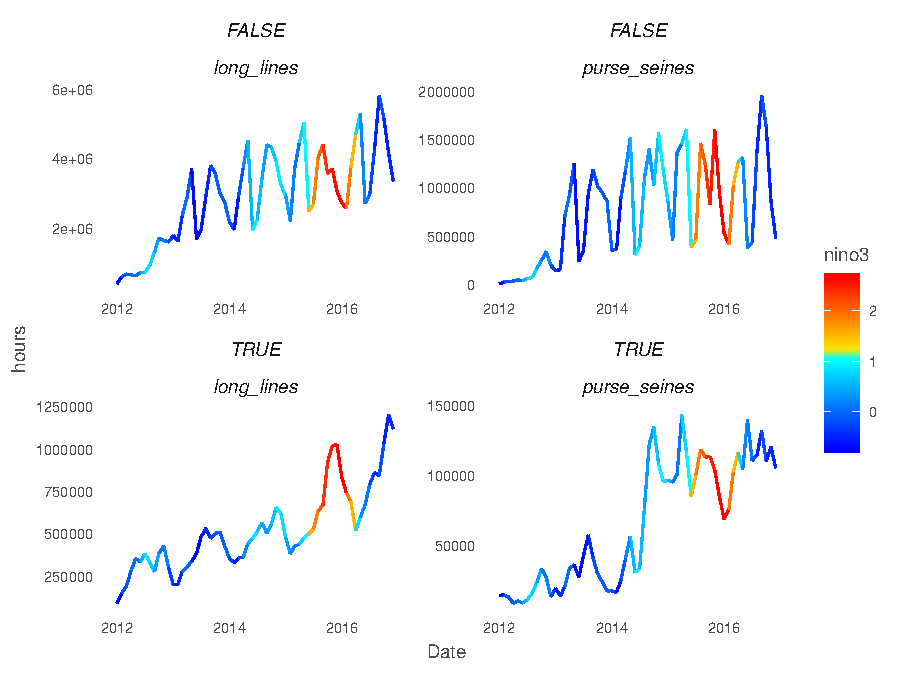
\includegraphics{img/trends_by_gear.pdf}
\caption{Trends in fishing hours by gear and foreign}
\end{figure}

We estimate the effects of ENSO on Foreign Fishing using a difference-in-difference strategy to compare the effects of ENSO on foreign fishing in regions impacted by ENSO to its effects on foreign fishing in regions not impacted by ENSO. 

\begin{equation}
\label{eq_FF}
log(FF_{ct}) = \alpha + \beta ENSO_{t} \times \mathbb{I}_{c \epsilon T} + \phi_{t} + \lambda_{c} + \epsilon_{ct}
\end{equation}


\noindent $FF_{ct}$ represents the foreign fishing variable of interest by country and year. We use an inverse hyperbolic sine\footnote{$ln(FF+\sqrt{1+FF^2}) \xrightarrow{} ln(2L)$} of our foreign fishing variable in my main specification to transform zeroes in my data \cite{Burbidge:1988, Card:2017}. $\alpha$ is a constant and $\beta$ captures the linear effect of ENSO on countries in effected regions compared to counties in regions uneffected by ENSO. The treatment is ENSO interacted with a dummy, $\mathbb{I}_{c \epsilon T}$, that equals 1 for countries in ENSO-effected regions and 0 for counties in uneffected-ENSO regions. $\phi_{t}$ are monthly fixed effects and $\lambda_{c}$ are country fixed effects. Standard errors are clustered at the country level.

\subsubsection{Empirical specifications: Identify treatment regions}
\label{Treatment}
First we established a relationship between ENSO and two local environmental variables that drive the geographical presence of fish stocks, sea-surface temperature (SST) and windspeed. We obtain an average monthly SST value, $SST_{t}$, for each grid-point from the NOAA OI SST Dataset within the spatial bounds of each fishery as defined by the NEFSC (see fig. 1 in main text). We run the following regression model:

NOTE: WE MAY NOT NEED TO DETREND SST
\begin{equation}
\label{eq_SI_SST}
SST_{t} = \omega + \phi ENSO_{t} + \sum_{p=1}^{N} \mu_{p} t^p + \epsilon_{t} 
\end{equation}  

\noindent where $\omega$ is a constant, $\phi$ captures the linear effect of monthly ENSO and $\mu_{p}$ captures the effect of a pth-order polynomial time trend. Standard errors use the Newey-West adjustment which allows for serial correlation and heteroscedasticity of arbitrary form in the error terms over an optimally chosen window of time \cite{Newey:1987, Newey:1994}. SST during this sample period exhibited trending behavior and thus needed to be detrended. To determine the polynomial order of the time trend, $N$, we use the Akaike Information Criteria (AIC) \cite{Akaike:1974}, which when minimized captures a model's overall goodness of fit while penalizing additional terms with limited explanatory power. For both fisheries, we observe that the AIC statistic drops when a time trend of second-order or higher is included in Equation \ref{eq_SI_SST}. Importantly, we detect a positive/negative relationship between winter ENSO and SST and a positive/negative relationship between winter ENSO and windspeed, shown in Figure \ref{}.

\begin{equation}
\label{eq_T}
log(FF_{t}) = \psi + \delta ENSO_{t} + \sum_{p=1}^{N} \kappa_{p} t^p + \mu_{t}
\end{equation}

\noindent $\psi$ is a constant; $\delta$ captures the linear effect of ENSO and $\kappa_{p}$ represents the effect of a $p^{th}$-order polynomial time trend. Standard errors use the Newey-West adjustment, allowing for arbitrary forms of serial correlation and heteroscedasticity in the error term with a bandwidth of 10 months. As a robustness check, we use different polynomial time trends to remove any long-term trends.

\begin{figure}
\centering
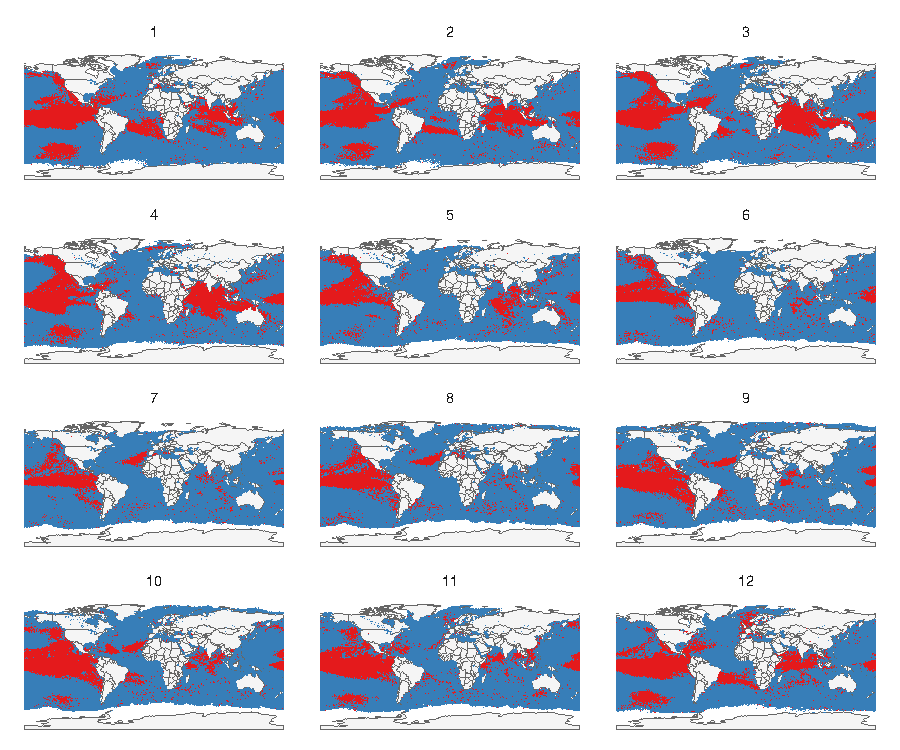
\includegraphics{img/cor_sst_nino34.pdf}
\caption{Monthly correlations between SST and nino3 index. Numbers above each pannel indicate the month (1 = Jan, 12 = Dec).
Red zones indicate the pearson's correlation coefficient was \textgreater{} 0 and p \textless{} 0.1.}
\end{figure}

\begin{figure}
\centering
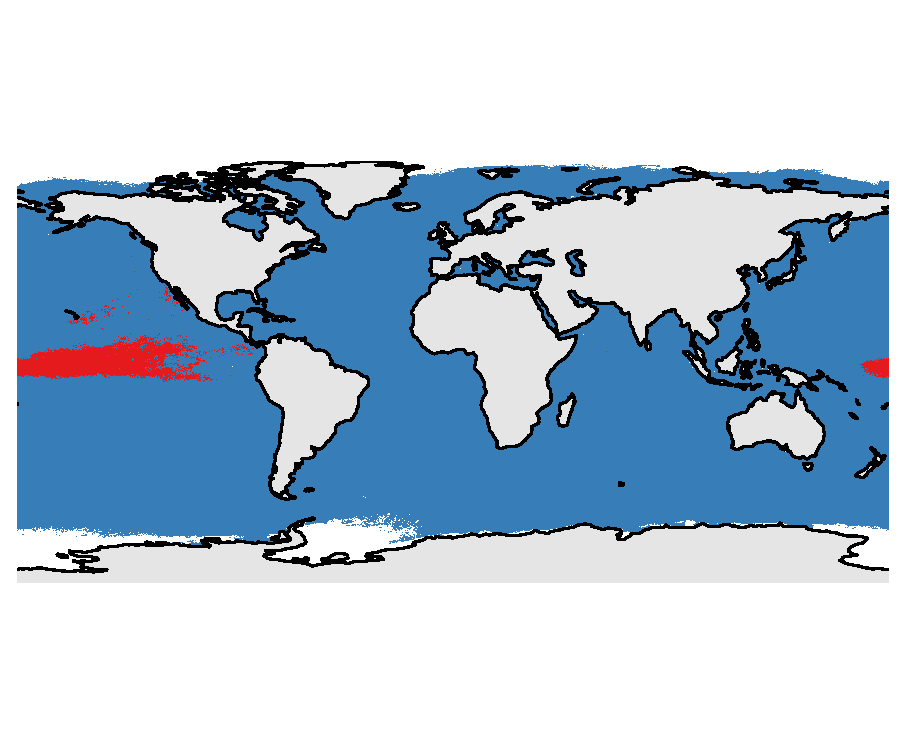
\includegraphics{img/cor_sst_nino34_var.pdf}
\caption{ENSO teleconnection depending on number of months. Number above figures indicate the minimum number of months for which a particular
parcel was correlated to nino3 (red). For example, the panel 6 indicates that all red regions where SST showed a positive ( r \textgreater{} 0)
and significant (p \textless{} 0.1) correlation with nino3 index for at least 6 months.}
\end{figure}




\newpage

\bibliography{references}

%% Here is the endmatter stuff: Supplementary Info, etc.
%% Use \item's to separate, default label is "Acknowledgements"

% \paragraph{Supplementary Information} is linked to the online version of the paper at www.nature.com/nature
 \paragraph{Acknowledgements} We thank Christopher Costello and Steve Gaines for their helpful comments and suggestions.
% \paragraph {Author information} The author declares that they have no competing financial interests. Correspondence and requests for materials
should be addressed to (email: ).



\end{document}
